\subsection{Arquitectura Flux}

La arquitectura Flux \cite{flux} es una de las grandes alternativas al patrón MVC \cite{mvc} en los últimos años en el ámbito del Front-End \cite{frontend}. Flux propone una arquitectura en la que el flujo de datos es unidireccional, donde estos viajan desde la vista por medio de acciones, llegando al {\it Store}, siendo actualizada la vista de nuevo.

\begin{figure}[H]
\centerline{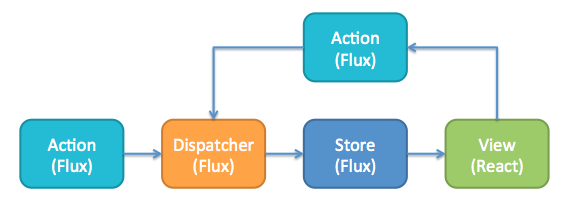
\includegraphics[width=15cm]{figuras/diseño/Flux.png}}
\caption{Modelo de funcionamiento de Flux.}
\label{enlaceImagenFlux}
\end{figure}

Como se puede observar en la \hyperref[enlaceImagenFlux]{Figura 3.5}, Flux está conformado por tres componentes, que llevan a cabo una acción. Estos son:
\begin{itemize}
    \item {\it Dispatcher} (disparador): Se encarga de identificar la acción a realizar y modificar los Stores afectados por la acción.
    \item {\it Store} (modelo de datos): Cada uno de los datos almacenados.
    \item {\it View} (vista): Componentes web que permiten la representación de los Store. Cada vez que se actualiza algo en el Store, la vista es actualizada.
\end{itemize}

La ventaja de todo ello es que al almacenarse los datos en un único lugar (denominado {\it estado}), resulta más sencillo depurar errores y saber qué está ocurriendo en cada situación.